\documentclass[11pt]{sigplanconf}

% The following \documentclass options may be useful:

% preprint      Remove this option only once the paper is in final form.
% 10pt          To set in 10-point type instead of 9-point.
% 11pt          To set in 11-point type instead of 9-point.
% authoryear    To obtain author/year citation style instead of numeric.

\usepackage{graphicx}

\begin{document}

\special{papersize=8.5in,11in}
\setlength{\pdfpageheight}{\paperheight}
\setlength{\pdfpagewidth}{\paperwidth}

\conferenceinfo{CONF 'yy}{Month d--d, 20yy, City, ST, Country} 
\copyrightyear{2014} 
\copyrightdata{978-1-nnnn-nnnn-n/yy/mm} 
\doi{nnnnnnn.nnnnnnn}

\titlebanner{Preprint.  Please do not redistribute}        % These are ignored unless
\preprintfooter{Preprint.  Please do not redistribute}   % 'preprint' option specified.

\title{Multithreading in Modern Mobile and Desktop Applications}
\subtitle{Not Much Thread-Level Parallelism; Lots of Event Handling}

\authorinfo{Name1}
           {Affiliation1}
           {Email1}
\authorinfo{Name2\and Name3}
           {Affiliation2/3}
           {Email2/3}

\maketitle

\begin{abstract}
This is the text of the abstract.
\end{abstract}

\category{CR-number}{subcategory}{third-level}

% general terms are not compulsory anymore, 
% you may leave them out
\terms
term1, term2

\keywords
keyword1, keyword2

\section{Introduction}

Multithreading is a commonplace feature of modern software.  Almost all
popular mobile and desktop applications create more than one thread at
some point.  Some applications keep dozens of threads alive.

It is a common misconception that the dominant purpose of threads in
modern software is taking advantage of the parallelism available in
multicore processors.  In fact, previous studies have found that most
applications exhibit very little thread-level parallelism (TLP).

We investigated this gap between the number of threads and the amount of
TLP.  Why are applications creating many threads, if they are not going
to take advantage of the available processors?  We find that the
majority of threads created by modern applications are what we call
\emph{event handler threads}.  Event handler (EH) threads spend the vast
majority of their lives blocked, waiting for some external event to
occur.  When the event happens, an EH thread becomes active very
briefly, then goes back to waiting for the next event.  Note that EH
threads are not structurally different from ``regular''
(i.e. long-running \emph{computation}) threads.  EH threads are defined
by a particular behavioral pattern.

This paper makes two contributions to the study of real-world
application multithreading behavior.  First, we extend previous TLP
studies to mobile platforms.  We find that mobile applications exhibit
marginally more TLP than desktop applications, but still very little.
Second, we quantify the extent to which applications use the event
handler thread pattern.

We are specifically \emph{not} interested in niche applications, some of
which make very good use of parallel computers.  We did this study to
inform the design of processors, programming languages and system
software.  The behavior of mainstream software is far more important
than niche software for these pieces of infrastructure, because that's
what drives the market.

The implications of our findings are significant for the industry going
forward.  Most applications are not getting involved in the multicore
revolution.  Researchers have proposed many approaches to improving the
benefit-to-pain ratio of parallel programming, but they have not yet had
a significant impact on the behavior of popular applications.  Unless
this changes there will be little demand for processors with more than a
few cores.

the second implication is related to the reliability of multithreaded
code.  Concurrency errors like data races and deadlocks are notorious
for causing sporadic and hard to fix defects in software.  Event handler
threads contribute negligibly to TLP, because they account for so little
run time.  Perhaps the functionality they implement should be done with
a different concurrency primitive that has better default bug avoidance
properties, like an event loop or .NET's async-await.

\section{Background and Related Work}

\section{Methods}

Use dynamic tracing tools to observe thread scheduling events.  See
table \ref{table:tracing-tools} for a summary.  These tools give us a
trace of all the thread scheduling events that happen during a
monitoring period.

\begin{table*}

\begin{tabular}{l|l|l}
System(s) & Tracing tool & Notes \\
\hline
Windows and Windows Phone & ETW (Event Tracing for Windows) & \\
Linux                     & FTrace                          & \\
Mac OS X and iOS          & Instruments (built on DTrace)   & \\
Android                   & Systrace                        & 
\end{tabular}
\caption{Platforms and tracing tools.}
\label{table:tracing-tools}
\end{table*}

\subsection{Thread-level parallelism}

Thread-level parallelism is intuitively a simple metric: how effectively
does an application use multiple processors?  Quantifying this concept
requires addressing two issues.  First, most applications have
significant idle periods, even when there user-level tasks ongoing.
Following previous thread behavior studies, we effectively ignore idle
time.  We are interested in how applications use processors when they
have something to do.  Idle time is not interesting.

Second, Not all activity ``belongs'' to a particular application.
During our experiments we took measures to limit extraneous activity,
but modern systems are complex, so completely eliminating unrelated
background processing is infeasible.  Further complicating this issue is
that some processing in processes not owned by a particular application
is actually done ``on behalf'' of that application.

For each test run we calculate a colletion of values $c_i$, the amount
of time that $i$ processors (cores) were actively used by an application
thread.  We calculate TLP as follows.

\begin{equation}
\mathrm{TLP} = \frac{\sum_{i=1}^N c_ii}{\sum_{i=1}^N c_i} \nonumber
\end{equation}

$N$ is simply the maximum number of threads that can run in parallel.
Notice that $c_0$ does not appear in either sum.  This is how we ignore
idle time.

\subsection{Event Handler Threads}

To quantify our notion of event handlers, we collected data on every
\emph{active interval} for every application thread.  An active interval
is simply the time between the system switching a thread onto a
processor and the system switching that thread off the processor.

We found that it is reasonably common for threads to be descheduled and
then rescheduled an extremely short time later.  We did not investigate
the reason for this behavior, but we decided to \emph{merge} these
adjacent active intervals when we found such gaps.  We used a maximum
gap length of 100 nanoseconds.

\section{Test Applications}

\section{Results}

We report two kinds of results: thread-level parallelism and ``event
handlerness''.

\subsection{Thread-Level Parallelism}

Our results are consistent with previous studies.  The amount of TLP
exhibited by the majority of applications is quite low.

\subsection{Event Handler Threads}

See figure \ref{figure:event_handler_data}.  The striking thing about
this data is that the majority of active intervals are extremely short
(less than one microsecond), yet the majority of processor time is
consumed by relatively long active persiods (more than 10 milliseconds).
This strongly supports the notion that there are two distinct uses of
threads in modern software: threads as units of parallel computation and
threads as mechanisms to make asyncronous/interactive software.

The applications were mostly consistent about this pattern, but there
was some variation, we pull out a couple of applications that were least
similar to the others and show them in figures X and Y.

\begin{figure}
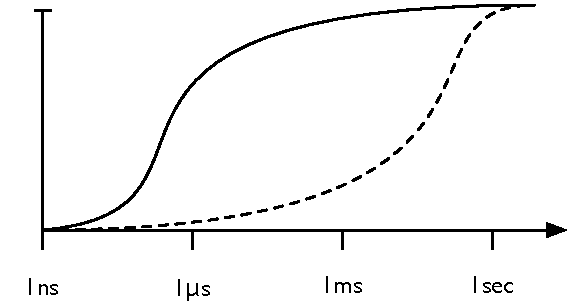
\includegraphics[width=\columnwidth]{cartoon_event_handler_data}
\caption{[Cartoon version!] The solid line is the cumulative number of
  active intervals that lasted less than a given amount of time.  The
  dashed line is cumulative amount of processor time accounted for by
  active intervals that lasted less than a given amount of time.  Note the
  time axis is scaled logarithmically.}
\label{figure:event_handler_data}
\end{figure}

\section{Discussion}

It appears that on mobile platforms the system does more work on behalf
of the applications.  We speculate that this is largely a result of
different security architectures.  Mobile operating systems give
applications less direct access to system services in an effort to
improve overall security.  One of the consequences of this is that it is
harder to properly account for which applications are using system
resources.  It may be useful to define an API to expose this
information.

Might have some implications for schedulers.

\section{Conclusions}

We explored two themes in this paper: most modern applications, both
mobile and desktop use very little thread-level parallelism.  As other
researchers have observed, unless this changes there will be very little
demand for processors with a large number of cores (``many-cores'').  We
believe that creative programmers would happily use more processor
power, if the price in development effort were right.  This suggests
that current tools for parallel programming do not make it sufficiently
appealing to the majority of developers.

The second theme is the event handler thread pattern.  We have shown
that EH threads are used pervassively in modern software, yet they have
received scant attention in the research literature.  It is possible
that applications would be better off using some primitive other than
threads (event loops, actors, cooperative threads, coroutines, \ldots).
It is also possible that system software developers could improve the
performance and/or bug resistance of applications by optimizing for
event handling, instead of only maximzing thread throughput.

\acks

Acknowledgments, if needed.

% We recommend abbrvnat bibliography style.

\bibliographystyle{abbrvnat}

% The bibliography should be embedded for final submission.

\begin{thebibliography}{}
\softraggedright

\bibitem[Smith et~al.(2009)Smith, Jones]{smith02}
P. Q. Smith, and X. Y. Jones. ...reference text...

\end{thebibliography}

\end{document}
